\documentclass{article}
\usepackage{graphicx}

\begin{document}


\title{INCALZIREA GLOBALA}
\author{ENACHE-DAVID NICOLETA}

\maketitle

\begin{abstract}
Aceasta lucrare prezinta aspecte pro si contra ale incalzirii globale.
Aceasta lucrare prezinta aspecte pro si contra ale incalzirii globale.
Aceasta lucrare prezinta aspecte pro si contra ale incalzirii globale.
\end{abstract}

\section{Introduction}
Here is the text of your introduction.....
\textbf{Astazi este duminica}
\underline{Totusi, avem cursuri online:)}

\begin{equation}
    \label{simple_equation}
    \alpha = \sqrt{ \beta }
\end{equation}

\section{Motivation}

\subsection{Subsection}
Write your subsection text here.

\subsection{Another subsection}
Write your subsection text here.


\begin{figure}
    
    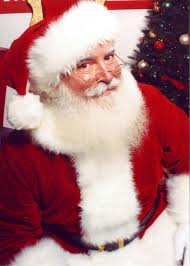
\includegraphics[width=3.0in]{mosul}
    \caption{Mos Craciun}
    \label{mosul}
\end{figure}

\section{Conclusion}
Write your conclusion here.

\end{document}